%%%%%%%%%%%%%%%%%%%%%%%%%%%%%%%%%%%%%%%%%
% Programming/Coding Assignment
% LaTeX Template
%
% This template has been downloaded from:
% http://www.latextemplates.com
%
% Original author:
% Ted Pavlic (http://www.tedpavlic.com)
%
% Note:
% The \lipsum[#] commands throughout this template generate dummy text
% to fill the template out. These commands should all be removed when 
% writing assignment content.
%
% This template uses a Perl script as an example snippet of code, most other
% languages are also usable. Configure them in the "CODE INCLUSION 
% CONFIGURATION" section.
%
%%%%%%%%%%%%%%%%%%%%%%%%%%%%%%%%%%%%%%%%%

%----------------------------------------------------------------------------------------
%	PACKAGES AND OTHER DOCUMENT CONFIGURATIONS
%----------------------------------------------------------------------------------------

\documentclass{article}

\usepackage{fancyhdr} % Required for custom headers
\usepackage{lastpage} % Required to determine the last page for the footer
\usepackage{extramarks} % Required for headers and footers
\usepackage[usenames,dvipsnames]{color} % Required for custom colors
\usepackage{graphicx} % Required to insert images
\usepackage{listings} % Required for insertion of code
\usepackage{courier} % Required for the courier font
\usepackage{lipsum} % Used for inserting dummy 'Lorem ipsum' text into the template

% Margins
\topmargin=-0.45in
\evensidemargin=0in
\oddsidemargin=0in
\textwidth=6.5in
\textheight=9.0in
\headsep=0.25in

\linespread{1.1} % Line spacing

% Set up the header and footer
\pagestyle{fancy}
\lhead{\hmwkAuthorName} % Top left header
\chead{\hmwkTitle} % Top center head
\rhead{\firstxmark} % Top right header
\lfoot{\lastxmark} % Bottom left footer
\cfoot{} % Bottom center footer
\rfoot{Page\ \thepage\ of\ \protect\pageref{LastPage}} % Bottom right footer
\renewcommand\headrulewidth{0.4pt} % Size of the header rule
\renewcommand\footrulewidth{0.4pt} % Size of the footer rule

\setlength\parindent{0pt} % Removes all indentation from paragraphs

%----------------------------------------------------------------------------------------
%	CODE INCLUSION CONFIGURATION
%----------------------------------------------------------------------------------------

\definecolor{MyDarkGreen}{rgb}{0.0,0.4,0.0} % This is the color used for comments
\lstloadlanguages{Perl} % Load Perl syntax for listings, for a list of other languages supported see: ftp://ftp.tex.ac.uk/tex-archive/macros/latex/contrib/listings/listings.pdf
\lstset{language=Perl, % Use Perl in this example
        frame=single, % Single frame around code
        basicstyle=\small\ttfamily, % Use small true type font
        keywordstyle=[1]\color{Blue}\bf, % Perl functions bold and blue
        keywordstyle=[2]\color{Purple}, % Perl function arguments purple
        keywordstyle=[3]\color{Blue}\underbar, % Custom functions underlined and blue
        identifierstyle=, % Nothing special about identifiers                                         
        commentstyle=\usefont{T1}{pcr}{m}{sl}\color{MyDarkGreen}\small, % Comments small dark green courier font
        stringstyle=\color{Purple}, % Strings are purple
        showstringspaces=false, % Don't put marks in string spaces
        tabsize=5, % 5 spaces per tab
        %
        % Put standard Perl functions not included in the default language here
        morekeywords={rand},
        %
        % Put Perl function parameters here
        morekeywords=[2]{on, off, interp},
        %
        % Put user defined functions here
        morekeywords=[3]{test},
       	%
        morecomment=[l][\color{Blue}]{...}, % Line continuation (...) like blue comment
        numbers=left, % Line numbers on left
        firstnumber=1, % Line numbers start with line 1
        numberstyle=\tiny\color{Blue}, % Line numbers are blue and small
        stepnumber=5 % Line numbers go in steps of 5
}

% Creates a new command to include a perl script, the first parameter is the filename of the script (without .pl), the second parameter is the caption
\newcommand{\perlscript}[2]{
\begin{itemize}
\item[]\lstinputlisting[caption=#2,label=#1]{#1.pl}
\end{itemize}
}

%----------------------------------------------------------------------------------------
%	DOCUMENT STRUCTURE COMMANDS
%	Skip this unless you know what you're doing
%----------------------------------------------------------------------------------------

% Header and footer for when a page split occurs within a problem environment
\newcommand{\enterProblemHeader}[1]{
\nobreak\extramarks{#1}{#1 continued on next page\ldots}\nobreak
\nobreak\extramarks{#1 (continued)}{#1 continued on next page\ldots}\nobreak
}

% Header and footer for when a page split occurs between problem environments
\newcommand{\exitProblemHeader}[1]{
\nobreak\extramarks{#1 (continued)}{#1 continued on next page\ldots}\nobreak
\nobreak\extramarks{#1}{}\nobreak
}

\setcounter{secnumdepth}{0} % Removes default section numbers
\newcounter{homeworkProblemCounter} % Creates a counter to keep track of the number of problems

\newcommand{\homeworkProblemName}{}
\newenvironment{homeworkProblem}[1][Problem \arabic{homeworkProblemCounter}]{ % Makes a new environment called homeworkProblem which takes 1 argument (custom name) but the default is "Problem #"
\stepcounter{homeworkProblemCounter} % Increase counter for number of problems
\renewcommand{\homeworkProblemName}{#1} % Assign \homeworkProblemName the name of the problem
\section{\homeworkProblemName} % Make a section in the document with the custom problem count
\enterProblemHeader{\homeworkProblemName} % Header and footer within the environment
}{
\exitProblemHeader{\homeworkProblemName} % Header and footer after the environment
}

\newcommand{\problemAnswer}[1]{ % Defines the problem answer command with the content as the only argument
\noindent\framebox[\columnwidth][c]{\begin{minipage}{0.98\columnwidth}#1\end{minipage}} % Makes the box around the problem answer and puts the content inside
}

\newcommand{\homeworkSectionName}{}
\newenvironment{homeworkSection}[1]{ % New environment for sections within homework problems, takes 1 argument - the name of the section
\renewcommand{\homeworkSectionName}{#1} % Assign \homeworkSectionName to the name of the section from the environment argument
\subsection{\homeworkSectionName} % Make a subsection with the custom name of the subsection
\enterProblemHeader{\homeworkProblemName\ [\homeworkSectionName]} % Header and footer within the environment
}{
\enterProblemHeader{\homeworkProblemName} % Header and footer after the environment
}

%----------------------------------------------------------------------------------------
%	NAME AND CLASS SECTION
%----------------------------------------------------------------------------------------

\newcommand{\hmwkTitle}{Programming\ Exercise\ \#1} % Assignment title
\newcommand{\hmwkDueDate}{Monday,\ January\ 1,\ 2012} % Due date
\newcommand{\hmwkClass}{Advanced\ Data\ Structures\ COL702} % Course/class
\newcommand{\hmwkClassTime}{10:30am} % Class/lecture time
\newcommand{\hmwkClassInstructor}{S.N.Maheshwari} % Teacher/lecturer
\newcommand{\hmwkAuthorName}{Anupam Sobti} % Your name

%----------------------------------------------------------------------------------------
%	TITLE PAGE
%----------------------------------------------------------------------------------------

\title{
\vspace{2in}
\textmd{\textbf{\hmwkClass\newline \hmwkTitle}}\\
\vspace{0.1in}\large{\textit{\hmwkClassInstructor}}
\vspace{3in}
}

\author{\textbf{\hmwkAuthorName}}
\date{2015ANZ8497} % Insert date here if you want it to appear below your name

%----------------------------------------------------------------------------------------

\begin{document}

\maketitle

%----------------------------------------------------------------------------------------
%	TABLE OF CONTENTS
%----------------------------------------------------------------------------------------

%\setcounter{tocdepth}{1} % Uncomment this line if you don't want subsections listed in the ToC

\newpage
\tableofcontents
\newpage

%----------------------------------------------------------------------------------------
%	PROBLEM 1
%----------------------------------------------------------------------------------------

% To have just one problem per page, simply put a \clearpage after each problem

\begin{homeworkProblem}
%Listing \ref{homework_example} shows a Perl script.

%\perlscript{homework_example}{Sample Perl Script With Highlighting}

%\lipsum[1]
Explain the insertion/deletion and access operations in 2-3 Trees.

\medskip

\problemAnswer{
Data is maintained on leaf nodes and the discriminant values are maintained on the internal nodes of the tree. An internal node has two values, known as discriminant values. The first value represents the largest value in the left subtree and the second value represents the largest value in the middle subtree if it exists.

\textbf{Search Operation: $Tree.search(x)$}\\
The function returns two values. The first value indicates whether or not the element was found (True/False). The second value is the position of the leaf containing $x$ or the leaf containing the value just greater than $x$. If $x$ is the greatest value in the tree, it returns the node whose child has the largest value in the already present tree. The algorithm states that the left child is traversed if $x < discrValue1$, else the middle child is traversed if $x < discrValue2$ if the discrValue2 exists. Otherwise, the right child is traversed. During the traversal if the node being traversed is a leaf, $x$ is compared to the data in leaf. If found equal, the search returns True,leafAddress else it returns False,leafAddress.
\medskip

\textbf{Insert Operation : }$Tree.insert(x)$\\
\textbf{Base Case:}\\
The first node is maintained as a leaf node. When the second value is inserted, one internal node is made the root which contains the smaller of the two leaves as the discriminant value.

\textbf{Insertion : Case 1}\\
Search for the node to be inserted. If the node is already present in the tree, the search returns (True,location of the node). In this case, there is no need for insertion since the element is already present.

\textbf{Insertion : Case 2}\\
The search returns the leaf node which is just greater than the element to be inserted, say \textit{y}. Case 2 represents the case where the parent of the leaf node returned contains two children. In this case, the third child can be accomodated by the parent of \textit{y} itself. Say the parent of \textit{y} is \textit{p}. Let's say the order of children of \textit{p} is \textit{c1} \textless\ \textit{x} \textless\ \textit{y}. The middle child is therefore updated to \textit{x} and the second discriminant value is updated to \textit{x}.  Hence, \textit{p} now has three children and the insertion is complete.

\textbf{Insertion : Case 3}\\
The search returns the leaf \textit{y} whose parent \textit{p} has three children. Say the children of \textit{p} are in the order $x_1$ \textless\ $x_2$ \textless\ $x_3$ \textless\ $x$. A new node is instantiated, say $q$. The nodes $x_3$ and $x$ are made the children of $q$. The second discriminant value of \textit{p} is removed and $x_3$ is made the first discriminant value for $q$. $q$ is then recursively inserted into parent of $p$.

The data for non-leaf nodes is calculated as the largest value in the subtree rooted at the node. This ensures the discriminant values being maintained when recursively inserting nodes at non-leaf levels.

\medskip

\textbf{Deletion :} $Tree.delete(x)$\\
\textbf{Base Case : }\\
The base case is when there are only two leaves rooted at a node and one of the leaves is deleted. In this case, the remaining leaf is made the root and the pointer to the root is returned as the pointer of the new tree.

\textbf{Deletion : Case 1}\\
Case 1 is the case where the search operation returns the node $x$ whose parent has three children. In this case, one of the children can be deleted from the parent of $x$ while mainintaining the rest of the structure. If $x$ is the leftmost child, the middle child is made the left child and the discriminant value 1 is made equal to discriminant value 2. The discriminant value 2 is updated to None. If it is the middle child, the node is deleted and discriminant value 2 is updated to None. If it is the right child, the middle child is made the right child and the discriminant value 2 is made None.

}

\pagebreak

\problemAnswer{

\textbf{Deletion : Case 2}\\
Case 2 is the case where the node whose child has to be deleted has only 2 children. In this case, the node either needs to merge with it's sibling (case 2.1) or borrow an excess leaf from one of it's sibling (case 2.2). 	
In case 2.1, the parent of the node being deleted $(x)$ has a sibling with only 2 children. Therefore, it cannot lend another child to the parent of $x$. Therefore, keeping the children of $x$'s parent and it's siblings in order, the two sibling are merged to form a node with 3 children. The discriminant values are recalculated from the left and middle subtree (in this case, leaves). Since, the number of nodes has reduced, this has to be recursively done for the next level as well. In case 2.2, a sibling with three children dispenses one of it's children and the node from which $x$ is deleted comes back to 2 children. The discriminant values have to be recalculated for both the nodes.
	}
\end{homeworkProblem}

%----------------------------------------------------------------------------------------
%	PROBLEM 2
%----------------------------------------------------------------------------------------

\begin{homeworkProblem}
	
%\lipsum[2]
Explain the insert/delete/access operations in AVL Trees.

%\problemAnswer{
%\begin{center}
%
\includegraphics[width=0.75\columnwidth]{example_figure} % Example image
%\end{center}

%\lipsum[3-5]
%}
\medskip

\problemAnswer{
AVL Trees are said to be balanced if, for all the nodes in the tree, the difference in the heights of it's children is atmost 1. The heights of all the nodes are maintained on the nodes themselves as an attribute.

\medskip
\textbf{Search Operation : }$Tree.search(x)$\\
The search operation is similar to a binary search tree.
Till the element is not found or the node is null, make node it's left child if $x < value\ in\ node$ else make the node it's right child. Return true and the node reference if $x = value\ in\ node$ else return false and the node reference.

\medskip
\textbf{Insert Operation : }$Tree.insert(x)$\\
The insertion in AVL Trees is done by simply following the search path and appending the node when a null is encountered. Thereafter, any imbalance in the nodes is rectified with the help of rotations.
From the point of insertion, nodes are traversed upwards till the magnitude of difference in heights of the children of the node is at most 1. Let's say the difference is defined as the height of left child - the height of the right child. If the difference is positive, a right rotation has to be done (Rotations are discussed later) else if the difference is negative, a left rotation has to be done. The rotations are performed using three nodes, all of which exist on the path of traversal from the inserted node to the root.
There are two types of rotations : Zig-zig and Zig-zag (both left and right). The rotations are illustrated in the figure below:
\begin{center}
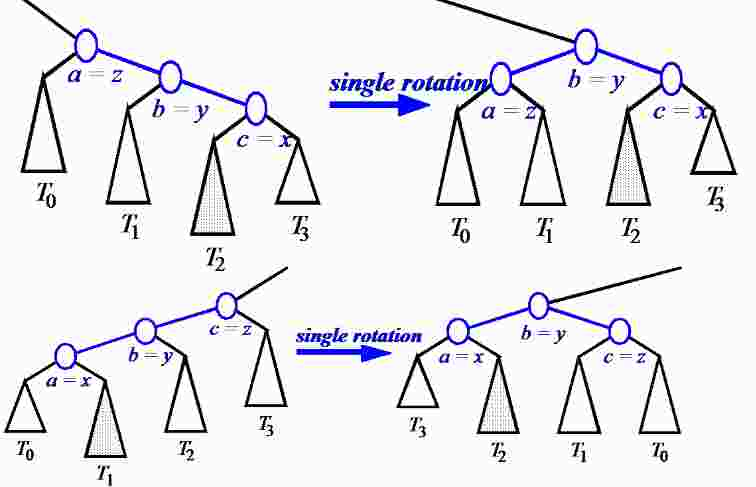
\includegraphics[width=0.75\columnwidth]{singleRotations} % Example image
\end{center}
}

\pagebreak
\problemAnswer{
\begin{center}
	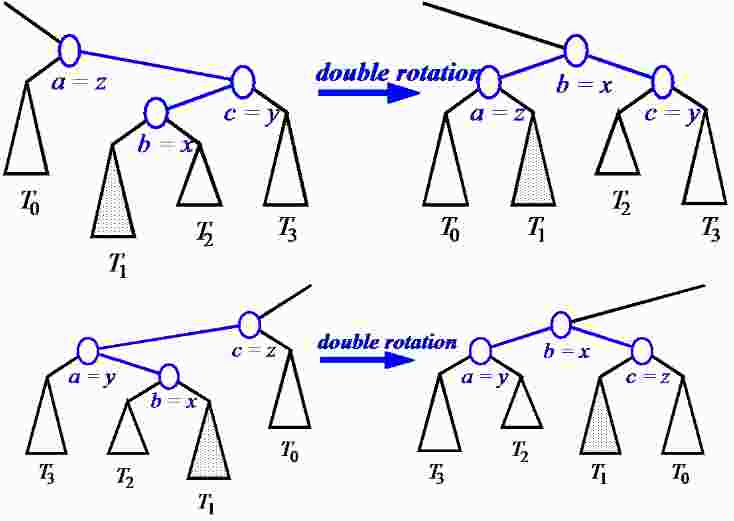
\includegraphics[width=0.75\columnwidth]{doubleRotations} % Example image
\end{center}
The heights of the nodes have to be updated after the rotation and the balance is restored.

\medskip
\textbf{Delete Operation : }\textit{Tree.delete(x)}\\
Let a node w is deleted. The reduction in height may cause the tree to be unbalanced. While moving towards the root from $w$, let $z$ be the node which is unbalanced. $y$ is the child of $z$ with greater height and $x$ is the child of $y$ with greater height. $x$,$y$ and $z$ will require a rotation similar to the rotations just discussed in order to bring the balance back at the root of this subtree (intially $z$). If the height of this subtree decreases after this rotation, the process has to be recursively done, going towards the root.
	}
\end{homeworkProblem}

%----------------------------------------------------------------------------------------
%	PROBLEM 3
%----------------------------------------------------------------------------------------

\newpage
\begin{homeworkProblem}
Explain insertion/deletion/search in Skip Lists.

\medskip
\problemAnswer{
Skip lists are arranged in a data structure where all the elements are present at the $0^{th}$ level in a doubly linked list. Now, roughly half of the these elements are stacked onto this level with vertical links to the elements on the $0^{th}$ level apart from the horizontally linked doubly linked list. This continues till $log(n)$ levels where $n$ is the number of elements in the list.

\medskip
\textbf{Search Operation : }$List.Search(x)$\\
The search operation begins at the topmost level. Let's say the current element under traversal is $e$. If $x < e$, we go to a level below the current level and go to the next element horizontally until $x \neq e$ or we are at the bottom level or $e$ is the first element in the list. The function returns $(True,e)$ if $x = e$; $(False,e)$ otherwise.

\medskip
\textbf{Insert Operation : }$List.Insert(x)$\\
The insert operation starts with a search operation for the element to be inserted. The search would return the element just greater than $x$ if $x$ isn't present already. The element is inserted at the bottom level and the height is then increased by 1 depending on the output of a random function which returns only 1s and 0s. If the function returns 1, the height is increased, meaning that the link for this element is contained in the level above the current level and linked with the element before and after the same. A similar process is then repeated for the next level until the random function outputs 0.

\medskip
\textbf{Delete Operation : }$List.Delete(x)$\\
The delete operation is carried out be firstly searching the element in the list. The node returned by the search operation is first deleted and then the deletion is carried out on the level above it if the element exists on the same. The maintained total number of elements determines the length of sentinels (towers bounding the elements in the list).
}
\end{homeworkProblem}

%----------------------------------------------------------------------------------------
%	PROBLEM 4
%----------------------------------------------------------------------------------------

\pagebreak
\begin{homeworkProblem}
Explain search/insert/delete operations in Red-Black Trees.

\medskip
\problemAnswer{
Data is maintained on the leaves and the internal nodes keep the discriminant values. The discriminant value is the largest value in the left subtree.

\medskip
\textbf{Search Operation : }$Tree.Search(x)$\\
The search operation is same as the binary search tree. Let the current node be $e$, then until $e$ is a leaf, $e = leftchild\ of\ e$ if $x \leq e$ else $e = rightchild\ of\ e$. If the leaf node = $x$, return $(True,leafNodeReference)$ else return $(False,leafNodeReference)$.

\medskip
\textbf{Insert Operation : }$Tree.Insert(x)$\\
Insertion begins with a search operation which returns the reference to the leaf whose parent will be the parent of $x$ when inserted. The insertion process is explained here synonymous to the insertion in 2-4 trees.\\
\textbf{Base Case}\\
A single value is maintained as a leaf. When another value is added, a black node is instantiated. The smaller of the two values becomes the left child and the larger becomes the right. The value in the node is the left child (discriminant value).\\
\textbf{Insertion Case 1}\\
When the leaf is to be inserted into a black colored node whose both children are black/leaves, a red node is instantiated. The three values (two existing nodes and $x$) are then made children of the red node and right child of the black node.\\
\textbf{Insertion Case 2}\\
When the leaf is to be inserted into a black node which has a black child and a red child, another red node is instantiated which is made the children of the black node. The newly inserted red node has the black child and $x$ as it's children.\\
\textbf{Insertion : Case 3}\\
When the leaf is to be inserted into a red node which has a red sibling, the red node is removed and one of the children of the red node are made the children of the black node which was the parent of the red node. Another black node is instantiated which is recursively inserted into the grandparent of the red node.\\

\medskip
\textbf{Deletion Operation : }$Tree.delete(x)$\\
\textbf{Deletion Case 1}\\
The node is found using the search operation. If the parent is a red node, the red node and the node returned by the search are deleted and the remaining child is made the direct child of the black node. The discriminant value is recalculated for the path of deletion until the discriminant value is equal to the already stored discriminant value.\\
\textbf{Deletion Case 2}\\
The parent of the node being deleted is black with the other child being red. The red node is deleted and the children of the red node are made the children of the black parent.\\
\textbf{Deletion Case 3}\\
The parent of the node being deleted is black with the other child being black. The sibling of the parent has a red child. The red node is deleted and of the children of the red node replaces the deleted node. The other child of the red node is made a direct child to the black parent of the red node.\\
}
\pagebreak
\problemAnswer{
\textbf{Deletion Case 4}\\
The parent of the node being deleted is black with the other child being black but the sibling of the parent doesn't have a red child. The parent of the node being deleted is deleted too. The other child of this parent is then made a child of a newly instantiated red node which is made the child of the black sibling. The other child of the sibling is the black node which was already it's child. Since this reduces the number of nodes of the grandchild, the process has to be recursively repeated.
	}
\end{homeworkProblem}
%----------------------------------------------------------------------------------------

\end{document}